In Versuchs 234 betrachten wir verschiedene Arten von Lichtquellen und deren Spektren. Hierbei unterscheiden wir speziell zwischen Temperaturstrahlern und Nichttemperaturstrahlern, welche in ihrer Art und Weise, Licht bzw. Strahlung auszusenden auf zwei verschiedenen physikalischen Phänomenen basieren.

\subsection{Physikalische Grundlagen}

Zur Erklärung von \textbf{Temperaturstrahlern} betrachten wir zunächst einen idelisierten schwarzen Körper, also einen Körper mit dem Emissionsvermögen $\varepsilon = 1$. Sobald die Temperatur $T$ dieses, und allgemein jedes Körpers, größer $0 \si{\kelvin}$ ist, sendet dieser elektromagnetische Strahlung aus, deren Intensität dem Planck'schen Strahlungsgesetz
\begin{align}
  M_{\lambda} (\lambda, T) \dd{A} \dd{\lambda} = \frac{2 \pi h c^2}{\lambda^5} \frac{1}{\e{\frac{hc}{\lambda k T}} - 1} \dd{A} \dd{\lambda}
\end{align}
folgt. $M_{\lambda}$ steht hierbei für die Strahlungsleistung, welche vom Flächenelement $\dd{A}$ im Wellenlängenbereich $\qty[\lambda, \lambda + \dd{\lambda}]$ abgestrahlt wird. Die Intensitätsverteilung besitzt ein Maximum bei einer bestimmten Wellenlänge, welche nach dem Wie'schen Verschiebungsgesetz
\begin{align}
  \lambda_{\max} = \frac{2897.8 \si{\micro\meter\kelvin}}{T}
\end{align}
von der Temperatur des Körpers abhängt.

Durch Betrachtung der Farbe des ausgestrahlten Lichts lassen sich dich Lichtquellen charakterisieren. Ein Körper erscheint bei einer Temperatur von $0\si{\kelvin}$ absolut schwarz. Darauf folgt bei leichter Erwärmung die Emission von zunächst rotem Licht. Bei einer weiteren Erwärmung wird zusätzlich grünes licht emittiert, welches sich mit den Rotanteilen zu orange bis gelblich erscheinendem Licht vermischt. Weißlich wirkendes Licht erhält man, wenn sich bei einer Temperatur von etwa $5500 \si{\kelvin}$ alle Wellenlängen des sichtbaren Bereichs mit etwa gleicher Intensität emittiert werden. Mit weiterer Erwärmung des Körpers kommen vermehrt Blauanteile hinzu, welche das Licht zunächst hellblau, dann blau bis violett erscheinen lässt.

Die Streuung von Licht ist nach der Rayleigh-Streuung stark Frequenzabhängig, daher wird blaues Licht deutlich stärker gestreut als rotes Licht. Dies ist auch der Grund, weshalb der Himmel blau erscheint, obwohl das direkte Sonnenlicht weiß ist. Betrachtet man das kontinuierliche Spektrum des von der Sonne abgestrahlten Lichts, so sind in diesem Absorptionslinien, die sogenannten Frauenhoferlinien zu erkennen. Diese entstehen dadurch, dass die Atmosphärenschichten der Sonne und der Erde, welche das Licht passiert, Teile der Strahlung absorbieren.
 
Bei \textbf{Nichttemperaturstrahlern} beruht die Aussendung von Licht auf der Anregung von Atomzuständen in Gasen oder Festkörpern oder der Rekombination von Elektron-Loch-Paaren in Halbleitern. Diese Art von Lichtquellen zeichnet sich durch diskrete Spektren, statt der kontinuierlichen bei Temperaturstrahlern, aus. Leuchtstoffröhren und Energiesparlampen sind Beispiele für Gasentladungslampen, die Quecksilberdampf als Leuchtgas verwenden. Da die meiste emittierte Strahlung von Quecksilber im nicht sichtbaren UV-Bereich liegt, werden derartige Lampen mit einem Leuchtstoff umzogen, welcher bei Bestrahlung mit UV-Licht im sichtbaren Bereich fluoresziert. In Leuchtdioden (LEDs) werden in pn-Übergängen bei der Rekombination von Elektron-Loch-Paaren Photonen emittiert. Die Farbe des Lichts hängt hierbei von den Halbleitermaterialien ab.

Neben den Quecksilberdampflampen sind Natriumdampflampen ein Beispiel für Gasentladungslampen, welche wir in diesem Versuch auch näher betrachten werden. Natrium ist ein Alkalimetall, dessen Atome ein Leuchtelektron besitzen. Das Potential, welches dieses eine Elektron \glqq{}sieht\grqq{}, kann in Kernnähe durch das Coulombpotential
\begin{align}
  V(r) = -\frac{Ze^2}{4 \pi \varepsilon_0 r}
\end{align}
und in weiterer Entfernung über das Wasserstoffpotential
\begin{align}
  V(r) = -\frac{e^2}{4 \pi \varepsilon_0 r}
\end{align}
angenähert werden. Dieses ist kein Coulombpotential mehr, somit ist die Entartung des Bahndrehimpuls $l$ aufgehoben und die Energieniveaus 
\begin{align}
  E_{n,l} = -13.6\si{\electronvolt} \frac{1}{(n - \Delta_{n,l})^2}
\end{align}
hängen neben der Hauptquantenzahl $n$ auch von der Bahndrehimpulsquantenzahl ab. Die Korrektur $\Delta_{l,n}$ kann aufgrund der geringen $n$-Abhängigkeit zu $\Delta_{l}$ umgeschrieben beziehungsweise angenähert werden. Halten wir die Hauptquantenzahl $n$ fest, so liegt das $s$-Niveau am tiefsten und das $d$-Niveau am höchsten. Die Übergänge $np\to3s$ werden als Hauptserie bezeichnet. Die Übergänge $nd\to3p$ und $ns\to3p$ bezeichnen wir als erste und zweite Nebenserie. Die wichtigsten Übergänge sind in \abbref{fig:uebergaenge} dargestellt.

\begin{figure}[H]
  \centering
  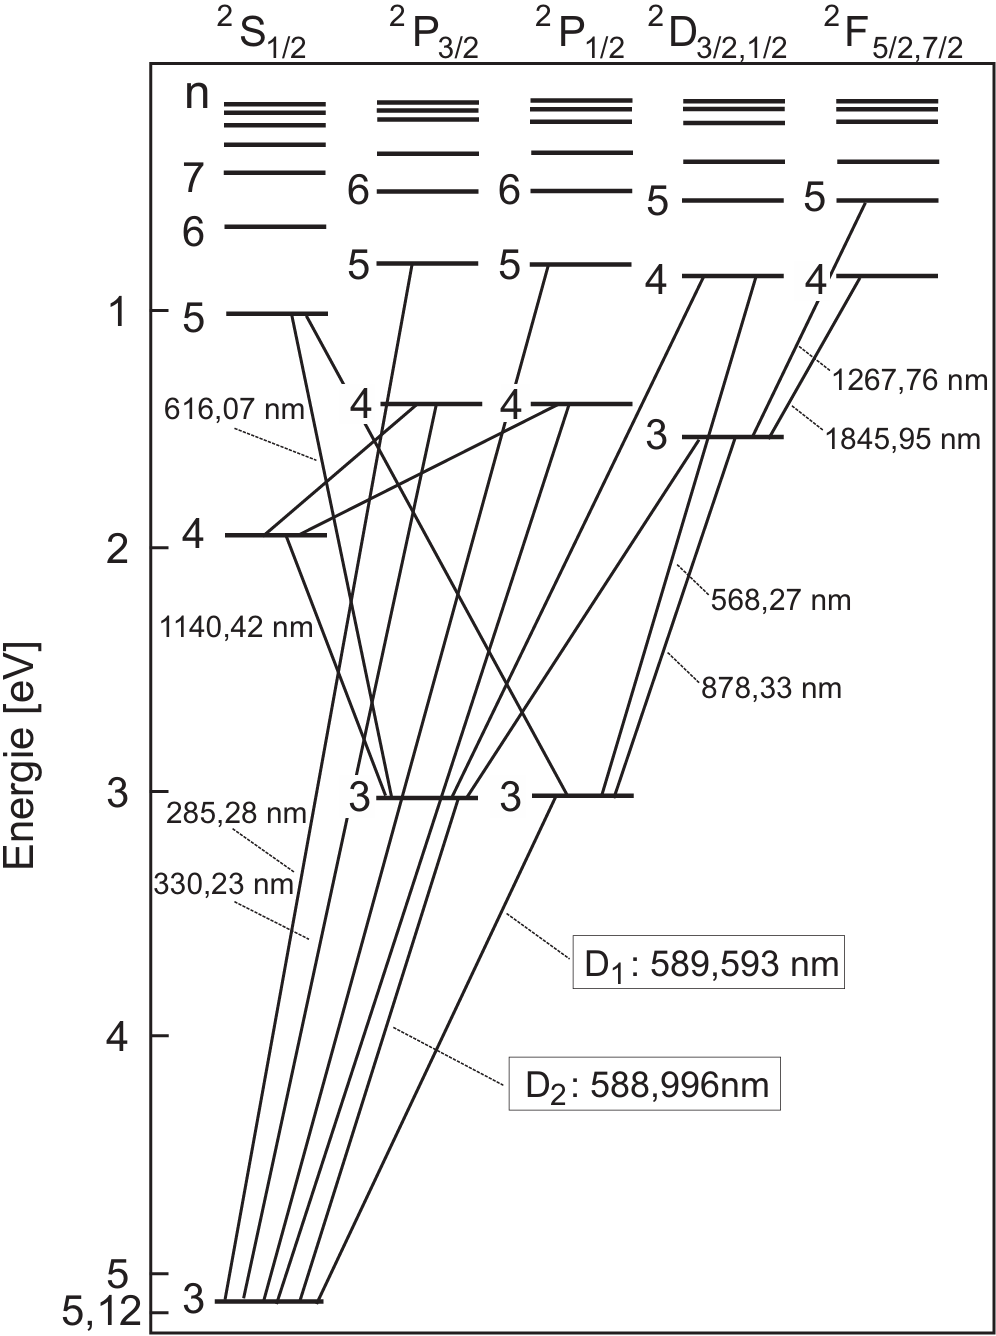
\includegraphics[width=0.5\textwidth]{files/uebergaenge.png}
  \caption{Energiespektrum und wichtige Übergänge im Natriumatom}
  \label{fig:uebergaenge}
\end{figure}

\newpage

\subsection{Versuchsdurchführung}